% vim: nu expandtab shiftwidth=2 softtabstop=2 autoindent foldmethod=marker
\documentclass{article}
\usepackage{fancyhdr}
\usepackage{multirow}   %helps with tables, allows for multiple rows to combine
\usepackage{amssymb}    %allows for the use of \square which makes a blank square in long multiplication
\usepackage[hidelinks, letterpaper, pagebackref, bookmarksopen, bookmarksnumbered]{hyperref} %makes table of contents
\usepackage{bookmark}                                                                        %helps with table of contents
\usepackage{import}
\usepackage{xcolor,colortbl} %lets me make colored rows and columns in tables
\usepackage{listings} %lets me input c++ code easily
\usepackage{pgfplots}

\def\mydate{\leavevmode\hbox{\the\year-\twodigits\month-\twodigits\day}}
\def\twodigits#1{\ifnum#1<10 0\fi\the#1}
\title{Everything you need to know for C455}
\date{\mydate}
\author{The defeated souls of 10,000 students}

\fancypagestyle{plain}
{
  \fancyhf{}
  \lfoot{\author{The defeated souls of 10,000 students}}
  \cfoot{\thepage}
  \rfoot{\date{\mydate}}
  \renewcommand{\headrulewidth}{0pt}
}
\pagestyle{plain}

\begin{document}
\maketitle
\newpage
\pdfbookmark[section]{\contentsname}{toc}
\tableofcontents
\listoftables

%\newpage
% vim: nu expandtab shiftwidth=2 softtabstop=2 foldmethod=marker

\section{Homework 1}
\begin{enumerate}
\item Prove by induction that for any positive integer n, \\
  {\Large $\sum\limits_{i=1}^{n}i^{3}=\frac{n^{2}(n+1)^{2}}{4}$}
    \begin{itemize}
    \item [] First we must prove the base case, in this problem, since n must be a positive integer, the base case is where n is equal to 1.
    \item [] {\Large $\sum\limits_{i=1}^{1}i^{3}=\frac{n^{2}(n+1)^{2}}{4}$}
    \item [] This equation becomes {\Large $\sum\limits_{i=1}^{1}i^{3}=\frac{1^{2}(1+1)^{2}}{4}$} in this base case.
    \item [] {\Large $\Leftrightarrow \sum\limits_{i=1}^{1}i^{3}=\frac{1(1+1)^{2}}{4}$}
    \item [] {\Large $\Leftrightarrow \sum\limits_{i=1}^{1}i^{3}=\frac{1(2)^{2}}{4}$}
    \item [] {\Large $\Leftrightarrow \sum\limits_{i=1}^{1}i^{3}=\frac{1*4}{4}$}
    \item [] {\Large $\Leftrightarrow \sum\limits_{i=1}^{1}i^{3}=\frac{4}{4}$}
    \item [] $\Leftrightarrow \sum\limits_{i=1}^{1}i^{3}=1$
    \item [] $\Leftrightarrow (1)^{3}=1$
    \item [] $\Leftrightarrow 1=1$
    \item Since 1 is equal to 1, we proved that the base case is true.
    \item Now is the induction step. Let k be an arbitrary integer greater than 1. Assume {\Large $\sum\limits_{i=1}^{k}i^{3}=\frac{k^{2}(k+1)^{2}}{4}$} We will prove that {\Large $\sum\limits_{i=1}^{k+1}i^{3}=\frac{(k+1)^{2}((k+1)+1)^{2}}{4}$}
    \item We have {\Large $\sum\limits_{i=1}^{k+1}i^{3}=\left( \sum\limits_{i=1}^{k}i^{3} \right) + (k+1)^{3}$}
    \item By the inductive assumption we have {\Large $\sum\limits_{i=1}^{k+1}i^{3}=\left(\frac{k^{2}(k+1)^{2}}{4} \right) + (k+1)^{3}$}
    \item [] {\Large $\sum\limits_{i=1}^{k+1}i^{3}=\left(\frac{k^{2}(k^{2}+2k+1)}{4} \right) + (k+1)^{3}$}
    \item Now we factor $k^{2}+2k+1$ into $(k+1)^{2}$
    \item [] {\Large $\Leftrightarrow \sum\limits_{i=1}^{k+1}i^{3}=\left(\frac{k^{2}(k+1)^{2}}{4} \right) + (k+1)^{3}$}
    \item [] {\Large $\Leftrightarrow \sum\limits_{i=1}^{k+1}i^{3}=\left(\frac{k^{2}(k+1)^{2}}{4} \right) + \frac{4(k+1)^{3}}{4}$}
    \item [] {\Large $\Leftrightarrow \sum\limits_{i=1}^{k+1}i^{3}=\left(\frac{k^{2}(k+1)^{2}+4(k+1)^{3}}{4} \right)$}
    \item [] {\Large $\Leftrightarrow \sum\limits_{i=1}^{k+1}i^{3}=\left(\frac{(k+1)^{2}(k^{2}+4(k+1)^{1}}{4} \right)$}
    \item [] {\Large $\Leftrightarrow \sum\limits_{i=1}^{k+1}i^{3}=\left(\frac{(k+1)^{2}(k^{2}+4k+4)}{4} \right)$}
    \item [] {\Large $\Leftrightarrow \sum\limits_{i=1}^{k+1}i^{3}=\frac{(k+1)^{2}(k+2)^{2}}{4}$}
    \item [] {\Large $\Leftrightarrow \sum\limits_{i=1}^{k+1}i^{3}=\frac{(k+1)^{2}((k+1)1)^{2}}{4}$}
    \item This proves that {\Large $\sum\limits_{i=1}^{k+1}i^{3}=\frac{(k+1)^{2}((k+1)+1)^{2}}{4}$} holds. By induction, {\Large $\sum\limits_{i=1}^{n}i^{3}=\frac{n^{2}(n+1)^{2}}{4}$} holds for all positive integers.
    \end{itemize}

\item In each case below, explain why the given expression is true:
  \begin{enumerate}
  \item $3n^{2} + 100n + \log{(n)} = O(n^{2})$
    \begin{itemize}
    \item [] First we use the limit theorem of Big O which states that $f(n)=O(g(n)) \Leftrightarrow \frac{f(n)}{g(n)} < \infty$.
    \item [] Hence {\Large $$\lim_{n \to \infty} \frac{3n^{2} +100n +\log{(n)}}{n^{2}} < \infty$$}
    \item [] {\Large $$\Leftrightarrow \lim_{n \to \infty} \frac{3n^{2}}{n^{2}} + \lim_{n \to \infty} \frac{100n}{n^{2}} + \lim_{n \to \infty} \frac{\log{(n)}}{n^{2}} < \infty$$}
    \item [] {\Large $$\Leftrightarrow \lim_{n \to \infty} 3 + \lim_{n \to \infty} \frac{100}{n} + \lim_{n \to \infty} \frac{\log{(n)}}{n^{2}} < \infty$$}
    \item [] Now we use the limit definion that says {\Large $$\lim_{n \to \infty} \frac{c}{n^{a}} =0$$} where c and a are positive constants.
    \item [] {\Large $$\Leftrightarrow \lim_{n \to \infty} 3 +0+ \lim_{n \to \infty} \frac{\log{(n)}}{n^{2}} < \infty$$}
    \item [] {\Large $$\Leftrightarrow \lim_{n \to \infty} 3 + \lim_{n \to \infty} \frac{\log{(n)}}{n^{2}} < \infty$$}
    \item [] Now we use the limit definition that says $$\lim_{n \to \infty} c = c$$ where c is some constant.
    \item [] Hence {\Large $$3 + \lim_{n \to \infty} \frac{\log{(n)}}{n^{2}} < \infty$$}
    \item [] Since we have a different base, we need to use the change of base formula for logarithms. $log_{b}x =ln(x)/ln(b)$
    \item [] Hence {\Large $$\Leftrightarrow 3 + \lim_{n \to \infty} \frac{\ln{(n)}}{\ln{2}*n^{2}} < \infty$$}
    \item [] Now, since $$\lim{n \to \infty} \ln{n} = \infty$$, and $$\lim_{n \to \infty} \ln{2}*n^{2} = \infty$$ we use lopitals rule and take the derivative. 
    \item [] Hence {\Large $$\Leftrightarrow 3 + \lim_{n \to \infty} \frac{1}{2\ln{2}*n^{2}} < \infty$$}
    \item [] Now we use the limit definion that says {\Large $$\lim_{n \to \infty} \frac{c}{n^{a}} =0$$} where c and a are positive.
    \item [] Hence {\Large $$\Leftrightarrow 3 + 0 < \infty$$}
    \item [] {\Large $$\Leftrightarrow 3 < \infty$$}
    \item As 3 is less than infinity, we have proved that $3n^{2} + 100n + \log{(n)} = O(n^{2})$
    \end{itemize}
  \item $(\sqrt{n} +1)^{8} = O(n^{4})$
    \begin{itemize}
    \item [] Begin by changing the exponent on n
    \item [] {\Large{$\Leftrightarrow (n^{\frac{1}{2}} +1)=O(n^{4})$}}
    \item [] Then expand the left side.
    \item [] {\Large{$\Leftrightarrow n^{4} + 8n^{\frac{7}{2}} +28n^{3} +56n^{\frac{5}{2}} + 70n^{2} +56n^{\frac{3}{2}} +28n +8n^{\frac{1}{2}} +1 = O(n^{4})$}}
    \item [] First we use the limit theorem of Big O which states that $f(n)=O(g(n)) \Leftrightarrow \frac{f(n)}{g(n)} < \infty$.
    \item [] {\Large{$$\Leftrightarrow \lim_{n \to \infty} \frac{n^{4} + 8n^{\frac{7}{2}} +28n^{3} +56n^{\frac{5}{2}} + 70n^{2} +56n^{\frac{3}{2}} +28n +8n^{\frac{1}{2}} +1}{n^{4}} < \infty$$}}
    \item [] $$\Leftrightarrow \lim_{n \to \infty} \frac{n^{4}}{n^{4}} + \lim_{n \to \infty} \frac{8n^{\frac{7}{2}}}{n^{4}} + \lim_{n \to \infty} \frac{28n^{3}}{n^{4}} + \lim_{n \to \infty} \frac{56n^{\frac{5}{2}}}{n^{4}} + \lim_{n \to \infty} \frac{70n^{2}}{n^{4}} + \lim_{n \to \infty} \frac{56n^{\frac{3}{2}}}{n^{4}} + \lim_{n \to \infty} \frac{n}{n^{4}} + \lim{n \to \infty} \frac{8n^{\frac{1}{8}}}{n^{4}} + \lim_{n \to \infty} \frac{1}{n^{4}} < \infty$$
    \item [] $$\Leftrightarrow \lim_{n \to \infty} 1 + \lim_{n \to \infty} \frac{8}{n^{\frac{1}{2}}} + \lim_{n \to \infty} \frac{28}{n} + \lim_{n \to \infty} \frac{56}{n^{\frac{3}{2}}} + \lim_{n \to \infty} \frac{70}{n^{2}} + \lim_{n \to \infty} \frac{56}{n^{\frac{5}{2}}} + \lim_{n \to \infty} \frac{1}{n^{3}} + \lim{n \to \infty} \frac{8}{n^{\frac{7}{2}}} + \lim_{n \to \infty} \frac{1}{n^{4}} < \infty$$
    \item [] Now we use the limit definition that says {\Large $$\lim_{n \to \infty} \frac{c}{n^{a}} =0$$} where c and a are positive constants.
    \item [] Hence {\Large{$$\lim_{n \to \infty} 1 +0+0+0+0+0+0+0+0 < \infty$$}}
    \item [] {\Large{$$\Leftrightarrow \lim_{n \to \infty} 1 < \infty$$}}
    \item [] Now we use the limit definition that says $$\lim_{n \to \infty} c = c$$ where c is some constant.
    \item [] $\Leftrightarrow 1 < \infty$
    \item As 1 is less than infinity, we have proved that $(\sqrt{n} +1)^{8} =O(n^{4})$
    \end{itemize}
  \end{enumerate}

\item Prove by contradiction that $100n+2\neq O(\sqrt{n})$
  \begin{itemize}
  \item Suppose that $100n+2 = O(\sqrt{n})$
  \item [] Then we can turn sqare root into a power using its definition.
  \item [] {\Large $100n+2 = O(n^{\frac{1}{2}})$}
    \item [] Now we use the limit theorem of Big O which states that $f(n)=O(g(n)) \Leftrightarrow \frac{f(n)}{g(n)} < \infty$.
  \item [] Hence {\Large $$\lim_{n \to \infty} \frac{100n+2}{n^{\frac{1}{2}}} < \infty$$}
  \item [] {\Large $$\Leftrightarrow \lim_{n \to \infty} \frac{100n}{n^{\frac{1}{2}}} + \lim_{n \to \infty} \frac{2}{n^{\frac{1}{2}}} < \infty$$}
  \item [] Now we use the limit definition that says {\Large $$\lim_{n \to \infty} \frac{c}{n^{a}} =0$$} where c and a are positive constats.
  \item [] Hence {\Large $$\lim_{n \to \infty} \frac{100n}{n^{\frac{1}{2}}} + 0 < \infty$$}
  \item [] {\Large $$\Leftrightarrow \lim_{n \to \infty} \frac{100n}{n^{\frac{1}{2}}} < \infty$$}
  \item [] Now we use the limit definition that says {\large $$\lim_{n \to \infty} n = \infty$$}
  \item [] Hence $\infty < \infty$
  \item As infinity is not less than infinity, we have proved by contradiction that $100n+2 \neq O(\sqrt{n})$
  \end{itemize}
\end{enumerate}


% vim: nu expandtab shiftwidth=2 softtabstop=2 foldmethod=marker

\documentclass{article}
\usepackage{fancyhdr}
\def\mydate{\leavevmode\hbox{\the\year-\twodigits\month-\twodigits\day}}
\def\twodigits#1{\ifnum#1<10 0\fi\the#1}
\title{Exam preparation Guide 1}
\date{\mydate}
\author{George Sparrow}

\fancypagestyle{plain}
{
  \fancyhf{}
  \lfoot{\author{George Sparrow}}
  \cfoot{\thepage}
  \rfoot{\date{\mydate}}
  \renewcommand{\headrulewidth}{0pt}
}
\pagestyle{plain}

\begin{document}
\maketitle
\newpage

Which of the following functions f(n) satifies $f(n)=O(n\log{(n)}$?
\begin{enumerate}
\item $f(n) = n^{2}-20n+\log{(n)}$
  \begin{itemize}
  \item First we use the limit definition of Big O notation that says $$\lim_{n \to \infty} \frac{f(n)}{g(n)} < \infty$$
  \item {\large $$\lim_{n \to \infty} \frac{n^{2}-20n+\log{(n)}}{n\log{(n)}} < \infty$$}
  \item Now we split the numerator using algebra.
  \item {\large $$\lim_{n \to \infty} \frac{n^{2}}{n\log{(n)}} - \lim_{n \to \infty} \frac{20n}{n\log{(n)}} +\lim_{n \to \infty} \frac{\log{(n)}}{n\log{(n)}} < \infty$$}
  \item Now we actually divide each of these.
  \item {\large $$\lim_{n \to \infty} \frac{n}{\log{(n)}} - \lim_{n \to \infty} \frac{20}{\log{(n)}} +\lim_{n \to \infty} \frac{1}{n} < \infty$$}
  \item Now we can use the limit definition that says $$\lim_{n \to \infty} \frac{1}{n^{a}} = 0$$, where a is some positive number.
  \item {\large $$\lim_{n \to \infty} \frac{n}{\log{(n)}} -0+0 < \infty$$}
  \item {\large $$\lim_{n \to \infty} \frac{n}{\log{(n)}} < \infty$$}
  \item Now, as the numerator and denominator both go to infinity as n goes to infinity, we need to use L'H$\hat{o}$pital's rule. So we take the derivative of the numerator and denominator.
  \item {\large $$\lim_{n \to \infty} \frac{1}{\frac{1}{n}} < \infty$$}
  \item {\large $$\lim_{n \to \infty} \frac{\frac{1}{1}}{\frac{1}{n}} < \infty$$}
  \item {\large $$\lim_{n \to \infty} n < \infty$$}
  \item Now we can use the limit definition that says $$\lim_{n \to \infty} n = \infty$$, where a is some positive number.
  \item {\large $$\infty < \infty$$}
  \item As infinity is not less than infinity (in this case since they are both the same infinity), this is a false statement.
  \end{itemize}
\item $f(n) = \log{(n!)}$
  \begin{itemize}
  \item First we use the limit definition of Big O notation that says $$\lim_{n \to \infty} \frac{f(n)}{g(n)} < \infty$$
  \item {\Large $$\lim_{n \to \infty} \frac{\log{(n!)}}{n\log{(n)}} <\infty$$}
  \item Now we use Stirlings approximation to replace $n!$ with $\sqrt{2n\pi}\left(\frac{n}{e}\right)^{n}$
  \item {\Large $$\lim_{n \to \infty} \frac{\log{(\sqrt{2n\pi}\left(\frac{n}{e}\right)^{n})}}{n\log{(n)}} <\infty$$}
  \item Now we use the multiplication rule of logarithms. $\log{a*b} = \log{a} + \log{b}$
  \item {\Large $$\lim_{n \to \infty} \frac{\log{(\sqrt{2n\pi})}}{n\log{(n)}} \lim_{n \to \infty} \frac{\log{(\left(\frac{n}{e}\right)^{n})}}{n\log{(n)}} <\infty$$}
  \item Now we use the rule of multiplication for square roots. $\sqrt{a*b} = \sqrt{a}*\sqrt{b}$
  \item {\Large $$\lim_{n \to \infty} \frac{\log{(\sqrt{2\pi})}}{n\log{(n)}} + \lim_{n \to \infty} \frac{\log{(\sqrt{n})}}{n\log{(n)}} + \lim_{n \to \infty} \frac{\log{(\left(\frac{n}{e}\right)^{n})}}{n\log{(n)}} <\infty$$}
  \item Now we use the definition of logarithm that says $\log{a^{n}} = n\log{a}$
  \item {\Large $$\lim_{n \to \infty} \frac{\log{(\sqrt{2\pi})}}{n\log{(n)}} + \lim_{n \to \infty} \frac{(\frac{1}{2})\log{(n)}}{n\log{(n)}} + \lim_{n \to \infty} \frac{n\log{(\frac{n}{e})}}{n\log{(n)}} <\infty$$}
  \item Now we actually divide these.
  \item {\Large $$\lim_{n \to \infty} \frac{\log{(\sqrt{2\pi})}}{n\log{(n)}} + \lim_{n \to \infty} \frac{1}{2n} + \lim_{n \to \infty} \frac{n\log{(\frac{n}{e})}}{n\log{(n)}} <\infty$$}
  \item Now we can use the limit definition that says $$\lim_{n \to \infty} \frac{1}{n^{a}} = 0$$, where a is some positive number.
  \item {\Large $$\lim_{n \to \infty} \frac{n\log{(\frac{n}{e})}}{n\log{(n)}} + 0 + 0 <\infty$$}
  \item {\Large $$\lim_{n \to \infty} \frac{n\log{(\frac{n}{e})}}{n\log{(n)}} <\infty$$}
  \item Now we use the division rule of logarithms. $\log{a/b} = \log{a} - \log{b}$
  \item {\Large $$\lim_{n \to \infty} \frac{n\log{(n)}}{n\log{(n)}} - \lim_{n \to \infty} \frac{n\log{(e)}}{n\log{(n)}} <\infty$$}
  \item Now we actually divide these.
  \item {\Large $$\lim_{n \to \infty} 1 - \lim_{n \to \infty} \frac{\log{(e)}}{\log{(n)}} <\infty$$}
  \item Now we can use the limit definition that says $$\lim_{n \to \infty} \frac{1}{n^{a}} = 0$$, where a is some positive number.
  \item {\Large $$\lim_{n \to \infty} 1 - 0 <\infty$$}
  \item Now we can use the limit definition that says $$\lim_{n \to \infty} c =c$$, where c is some constant.
  \item $$1 <\infty$$
  \item As 1 is less than infinity, this is a true statement.
  \end{itemize}
\item {\large $\frac{n!}{\log{(n)}}$}
  \begin{itemize}
  \item First we use the limit definition of Big O notation that says $$\lim_{n \to \infty} \frac{f(n)}{g(n)} < \infty$$
  \item {\large $$\lim_{n \to \infty} \frac{n!}{n\log{(n)}\log{(n)}} < \infty$$}
  \item Now we use Stirlings approximation to replace $n!$ with $\sqrt{2n\pi}(\frac{n}{e})^{n}$
  \item {\large $$\lim_{n \to \infty} \frac{\sqrt{2n\pi}(\frac{n}{e})^{n}}{n\log{(n)}\log{(n)}} < \infty$$}
  \item Now we use the rule of multiplication for square roots. $\sqrt{a*b} = \sqrt{a}*\sqrt{b}$
  \item {\large $$\lim_{n \to \infty} \frac{\sqrt{2\pi}\sqrt{n}(\frac{n}{e})^{n}}{n\log{(n)}\log{(n)}} < \infty$$}
  \item Now we actually divide.
  \item {\large $$\lim_{n \to \infty} \frac{\sqrt{2\pi}(\frac{n}{e})^{n}}{n^{\frac{1}{2}}\log{(n)}\log{(n)}} < \infty$$}
  \item Now we split $\frac{n}{e}^{n}$ into $n^{n}$ and $e^{-n}$.
  \item {\large $$\lim_{n \to \infty} \frac{\sqrt{2\pi}e^{-n}n^{n-\frac{1}{2}}}{\log{(n)}\log{(n)}} < \infty$$}
  \item Now, as the numerator and denominator both go to infinity as n goes to infinity, we need to use L'H$\hat{o}$pital's rule. So we take the derivative of the numerator and denominator.
  \item {\Large $$\lim_{n \to \infty} \frac{e^{-n}n^{n-\frac{3}{2}}(\sqrt{2\pi}n\log{(n)}-\frac{\sqrt{2\pi}}{2})}{\frac{2\log{(n)}}{n}}$$}
  \item Now we simplify.
  \item {\Large $$\lim_{n \to \infty} \frac{\sqrt{2\pi}e^{-n}n^{n-\frac{3}{2}}(n\log{(n)}-\frac{1}{2})}{\frac{2\log{(n)}}{n}}$$}
  \item {\Large $$\lim_{n \to \infty} \frac{\sqrt{2\pi}e^{-n}n^{n-\frac{1}{2}}(n\log{(n)}-\frac{1}{2})}{2\log{(n)}}$$}
  \end{itemize}
\item $f(n) = \sqrt{n^{3}+1}$
\end{enumerate}
\end{document}


% vim: nu expandtab shiftwidth=2 softtabstop=2 foldmethod=marker

\documentclass{article}
\usepackage{fancyhdr}
\def\mydate{\leavevmode\hbox{\the\year-\twodigits\month-\twodigits\day}}
\def\twodigits#1{\ifnum#1<10 0\fi\the#1}
\title{Homework 2}
\date{\mydate}
\author{George Sparrow}

\fancypagestyle{plain}
{
  \fancyhf{}
  \lfoot{\author{George Sparrow}}
  \cfoot{\thepage}
  \rfoot{\date{\mydate}}
  \renewcommand{\headrulewidth}{0pt}
}
\pagestyle{plain}

\begin{document}
\maketitle
\newpage

\begin{enumerate}
\item For each recurrence relation below, determine if it is linear. If it it linear, determine all the non-zero coefficients and the nonhomogeneous term (if exists) of the recurrence relation.
  \begin{enumerate}
  \item $A_{n}=2A_{n-1}+2^{n}$
    \begin{itemize}
    \item [] All things in the form $$F_{n}=f(n) \sum\limits_{i=1}^{n}c_{i}(n)F_{n-i}$$ are linear recurrrence relations.
    \item In this case, $f(n)=2^{n}$, and $c=2$, so $$F_{n}=2^{n} \sum\limits_{i=1}^{n}2F_{n-i}$$ thus it is a linear reccurence relation. The non-zero coefficient is $2$ and the nonhomogenous term is $2^{n}$
    \end{itemize}
  \item $A_{n}=\log{(n)}A_{n-2}+3A_{n-3}$
    \begin{itemize}
    \item In this case it is a linear recurrence relation and the non-zero coefficients are $\log{(n)}$ and $3$, and there is no nonhomogenous term.
    \end{itemize}
  \item {\Large $A_{n}=\frac{A_{n-1}}{A_{n-2}}+1$}
    \begin{itemize}
    \item In this case, it is not a linear recurrence relation because they previous terms are dividing each other. The nonhomogenous term is $1$
    \end{itemize}
  \end{enumerate}
\item Check that the recurrence relation
  \begin{equation}
  F_{n}=6F_{n-1}-9F_{n-2}
  \end{equation}
has the following solution:
  \begin{equation}
  F_{n}=(\alpha_{1}+\alpha_{2}n)3^{n}
  \end{equation}
where $\alpha_{1}$ and $\alpha_{2}$ are any constants.
  \begin{itemize}
  \item [] In order to prove that this (equation 2) is a solution to the recurrence relation (equation 1), we substitute it (into equation 1) in order to attempt to get an identity (equation 2).
  \item $6((\alpha_{1}+\alpha_{2}(n-1))3^{(n-1)}) -9((\alpha_{1}+\alpha_{2}(n-2))3^{(n-2)})$
  \item [$\Leftrightarrow$]$2((\alpha_{1}+\alpha_{2}(n-1))3^{(n)}) -((\alpha_{1}+\alpha_{2}(n-2))3^{(n)})$
  \item [$\Leftrightarrow$]$3^{n}(2(\alpha_{1}+\alpha_{2}(n-1)) -(\alpha_{1}+\alpha_{2}(n-2)))$
  \item [$\Leftrightarrow$]$3^{n}(2\alpha_{1}+2n\alpha_{2}-2\alpha_{2} -\alpha_{1}-n\alpha_{2}+2\alpha_{2})$
  \item [$\Leftrightarrow$]$3^{n}(\alpha_{1}+n\alpha_{2})$
  \item [] through the commutative property of multiplication, which says that $ab=ba$, we get
  \item $(\alpha_{1}+\alpha_{2}n)3^{n}$
  \item As this is equation 2, we have the identity which proves that equation 2 is a solution to equation 1.
  \end{itemize}

\item Find the solution to each recurrence relation below.
  \begin{enumerate}
  \item $A_{0}=-2$; $A_{n}=3A_{n-1}$ for all $n\geq1$.
    \begin{itemize}
    \item [] Using the general solution for all linear homogenous first order recurrence relations, $F_{n}=A_{0}*c^{n}$ we get
    \item $A_{n}=(-2)*3^{n}$
    \item [] In order to prove that this ($A_{n}=-2*3^{n}$) is a solution to the recurrence relation ($3A_{n-1}$), we substitute it (into $3A_{n-1}$) in order to attempt to get an identity.
    \item $3(-2*3^{(n-1)})$
    \item [$\Leftrightarrow$]$-2*3*3^{(n-1)})$
    \item [$\Leftrightarrow$]$-2*3^{n})$
    \item As this is $-2*3^{n}$, we have the identity which proves that $2*3^{n}$ is a solution to $3A_{n-1}$
    \end{itemize}
  \item $B_{0}=1$; $B_{1}=8$; $B_{n}=B_{n-1}+2B_{n-2}$ for all $n\geq2$
    \begin{itemize}
    \item [] First, we need to place it in the form $Ax^{2}-Bx-C$, the characteristic equation.
    \item $x^{2}-x-2$
    \item [] Now we use the formula {\Large $x=\frac{-b \pm \sqrt{b^{2}-4ac}}{2a}$}
    \item {\Large $x=\frac{1 \pm \sqrt{1-4(1)(-2)}}{2}$}
    \item [$\Leftrightarrow$]{\Large $x=\frac{1 \pm \sqrt{1+8}}{2}$}
    \item [$\Leftrightarrow$]{\Large $x=\frac{1 \pm \sqrt{9}}{2}$}
    \item [$\Leftrightarrow$]{\Large $x=\frac{1 \pm 3}{2}$}
    \item {\Large $x_{1}=\frac{1+3}{2}$}
    \item {\Large $x_{1}=\frac{4}{2}$}
    \item {\Large $x_{1}=2$}
    \item {\Large $x_{2}=\frac{1-3}{2}$}
    \item {\Large $x_{2}=\frac{-2}{2}$}
    \item {\Large $x_{2}=-1$}
    \item [] Since $x_{1}$ and $x_{2}$ are not equal, we use the formula \\
      $F_{n}=\alpha_{1}(x_{1})^{n}+\alpha_{2}(x_{2})^{n} $ for all $n\geq0$
    \item [] Now we create a system of equations to solve for $\alpha_{1}$ and $\alpha_{2}$
    \item $B_{0}=\alpha_{1}+\alpha_{2}=1$
    \item [] $B_{1}=\alpha_{1}x_{1}+2\alpha_{2}x_{2}=8$
    \item [] Now we can use substitution to solve for $\alpha_{1}$ and $\alpha_{2}$
    \item [] $\alpha_{1}=1-\alpha_{2}$
    \item [] $(1-\alpha_{2})x_{1} +2\alpha_{2}x_{2}=8$
    \item [$\Leftrightarrow$] $(1-\alpha_{2})(2) +2\alpha_{2}(-1)=8$
    \item [$\Leftrightarrow$] $2-2\alpha_{2} -2\alpha_{2}=8$
    \item [$\Leftrightarrow$] $2-4\alpha_{2}=8$
    \item [$\Leftrightarrow$] $-4\alpha_{2}=6$
    \item [$\Leftrightarrow$] $\alpha_{2}=-\frac{3}{2}$
    \item [] $\alpha_{1}=1-\alpha_{2}$
    \item [] $\alpha_{1}=1+\frac{3}{2}$
    \item [] $\alpha_{1}=\frac{5}{2}$
    \item $F_{n}=\frac{5}{2}(2)^{n}-\frac{3}{2}(-1)^{n} $ for all $n\geq0$
    \item [] In order to prove that this ($F_{n}=\frac{5}{2}(2)^{n}-\frac{3}{2}(-1)^{n}$) is a solution to the recurrence relation ($B_{n-1}+2B_{n-2}$), we substitute it into \\($B_{n-1}+2B_{n-2}$) in order to attempt to get an identity \\($F_{n}=\frac{5}{2}(2)^{n}-\frac{3}{2}(-1)^{n}$).
    \item [] $B_{n-1}+2B_{n-2}$
    \item [$\Leftrightarrow$] $(\frac{5}{2}(2)^{n-1}-\frac{3}{2}(-1)^{n-1})+2(\frac{5}{2}(2)^{n-2}-\frac{3}{2}(-1)^{n-2})$
    \item [$\Leftrightarrow$] $\frac{5}{2}(2)^{n-1}+\frac{3}{2}(-1)^{n})+2\frac{5}{2}(2)^{n-2}-2\frac{3}{2}(-1)^{n})$
    \item [$\Leftrightarrow$] $\frac{5}{2}(2)^{n-1}-\frac{3}{2}(-1)^{n})+2\frac{5}{2}(2)^{n-2}$
    \item [$\Leftrightarrow$] $\frac{5}{2}(2)^{n-1}-\frac{3}{2}(-1)^{n})+\frac{5}{2}(2)^{n-1}$
    \item [$\Leftrightarrow$] $2\frac{5}{2}(2)^{n-1}-\frac{3}{2}(-1)^{n})$
    \item [$\Leftrightarrow$] $\frac{5}{2}(2)^{n}-\frac{3}{2}(-1)^{n})$
    \item As this is $\frac{5}{2}(2)^{n}-\frac{3}{2}(-1)^{n}$, we have the identity which proves that $\frac{5}{2}(2)^{n}-\frac{3}{2}(-1)^{n}$ is a solution to $F_{n}=B_{n-1}+2B_{n-2}$
    \end{itemize}
  \end{enumerate}
\end{enumerate}
\end{document}


% vim: nu expandtab shiftwidth=2 softtabstop=2 foldmethod=marker

\documentclass{article}
\usepackage{fancyhdr}
\def\mydate{\leavevmode\hbox{\the\year-\twodigits\month-\twodigits\day}}
\def\twodigits#1{\ifnum#1<10 0\fi\the#1}
\title{Homework 3}
\date{\mydate}
\author{George Sparrow}

\fancypagestyle{plain}
{
  \fancyhf{}
  \lfoot{\author{George Sparrow}}
  \cfoot{\thepage}
  \rfoot{\date{\mydate}}
  \renewcommand{\headrulewidth}{0pt}
}
\pagestyle{plain}

\begin{document}
\maketitle
\newpage

\begin{enumerate}
\item Find the general solution in closed form to each recurrence relation. For full credits, you need to justify your answers (if you apply some theorem, you need to cite them).
  \begin{enumerate}
  \item $A_{n}=3A_{n-1}+2^{n}$
    \begin{itemize} %{{{
    \item The first step is to solve the linear homogeneous relation portion of this equation.
    \item $A_{n}=3A_{n-1}$
    \item [] All things in the form $F_{n}=cF_{n-1}$ for all $n\geq1$ where $c_{i}$ is a nonzero constant, are homogeneous linear recurrrence relations.
    \item [] The general solution to all first order linear homogenous recurrence relations is $F_{n}=F_{0}c^{n}$
    \item Given that c=3, and $F_{0}=A_{0}$ is not defined, the solution to the linear homogeneous relation is $A_{0}3^{n}$
    \item [*] In order to prove that this ($A_{0}3^{n}$) is a solution to the recurrence relation ($3A_{n-1}$), we substitute it (into $3A_{n-1}$) in order to attempt to get an identity ($A_{0}3^{n}$).
    \item [*] $3*(A_{0}3^{n-1})$
    \item [*] $A_{0}3^{n}$
    \item [*] Since we have the identity $A_{0}3^{n}$, $A_{0}3^{n}$ is a solution to $3A_{n-1}$
    \item Now we solve the homogeneous part. Let $A_{n}=c2^{n}$ 
    \item Since we have $A_{n}=c2^{n}$ we also have $A_{n-1}=c2^{n-1}$
    \item Now we substitue $A_{n-1}=c2^{n-1}$ and $A_{n}=c2^{n}$ into $A_{n}=3A_{n-1}+2^{n}$ in order to solve for c.
    \item $c2^{n}=3(c2^{n-1})+2^{n}$
    \item $c2^{n}=3c2^{n-1}+2^{n}$
    \item $c2^{n}-2^{n}=3c2^{n-1}$
    \item $2^{n}(c-1)=3c2^{n-1}$
    \item $2^{n}(c-1)=\frac{3c2^{n}}{2}$
    \item $(c-1)=\frac{3c}{2}$
    \item $2(c-1)=3c$
    \item $2c-2=3c$
    \item $2c=3c+2$
    \item $-1c=2$
    \item $c=-2$
    \item Since $c=-2$, this gives us $A_{n}=-2(2^{n})$ which gives us $A_{n}=-2^{n+1}$
    \item Now, we put it all together.
    \item $A_{0}3^{n}-2^{n+1}$
    \item [*] In order to prove that this ($A_{0}3^{n}-2^{n+1}$) is a solution to the nonhomogeneous recurrence relation ($A_{n}=3A_{n-1}+2^{n}$), we substitute it (into $3A_{n-1}+2^{n}$) in order to attempt to get an identity ($A_{0}3^{n}-2^{n+1}$)
    \item [*] $3(A_{0}3^{n-1}-2^{n-1+1})+2^{n}$
    \item [*] $3A_{0}3^{n-1}-3*2^{n-1+1}+2^{n}$
    \item [*] $3A_{0}3^{n-1}-3*2^{n}+2^{n}$
    \item [*] $A_{0}3^{n}-3*2^{n}+2^{n}$
    \item [*] $A_{0}3^{n}-2*2^{n}$
    \item [*] $A_{0}3^{n}-2^{n+1}$
    \item [*] Since we have the identity $A_{0}3^{n}-2^{n+1}$, $A_{0}3^{n}-2^{n+1}$ is a solution to $A_{n}=3A_{n-1}+2^{n}$
    \end{itemize} % }}}
  \item $A_{n}=3A_{n-1}+3^{n}$
    \begin{itemize} %{{{
    \item The first step is to solve the linear homogeneous relation portion of this equation.
    \item $A_{n}=3A_{n-1}$
    \item [] All things in the form $F_{n}=cF_{n-1}$ for all $n\geq1$ where $c_{i}$ is a nonzero constant, are homogeneous linear recurrrence relations.
    \item [] The general solution to all first order linear homogenous recurrence relations is $F_{n}=F_{0}c^{n}$
    \item Given that c=3, and $F_{0}=A_{0}$ is not defined, the solution to the linear homogeneous relation is $A_{0}3^{n}$
    \item [*] In order to prove that this ($A_{0}3^{n}$) is a solution to the recurrence relation ($3A_{n-1}$), we substitute it (into $3A_{n-1}$) in order to attempt to get an identity ($A_{0}3^{n}$).
    \item [*] $3*(A_{0}3^{n-1})$
    \item [*] $A_{0}3^{n}$
    \item [*] Since we have the identity $A_{0}3^{n}$, $A_{0}3^{n}$ is a solution to $3A_{n-1}$
    \item Now we solve the homogeneous part. Normally, we would let $A_{n}=c3^{n}$, however, in this case the base ($3$) is equal to the constant multiplier in the homogeneous portion ($3$), and so we use the formula provided in the notes that says when $c=b$ is true, then $nb^{n}$ is the solution. So the solution to the non-homogeneous part is $n3^{n}$
    \item Now, we put it all together.
    \item $A_{n}=A_{0}3^{n} + n3^{n}$
    \item [*] In order to prove that this ($A_{0}3^{n}+n3^{n}$) is a solution to the nonhomogeneous recurrence relation ($A_{n}=3A_{n-1}+3^{n}$), we substitute it (into $3A_{n-1}+3^{n}$) in order to attempt to get an identity ($A_{0}3^{n}+n3^{n}$)
    \item [*] $3(A_{0}3^{n-1} + (n-1)3^{n-1}) + 3^{n}$
    \item [*] $3A_{0}3^{n-1} + 3(n-1)3^{n-1} + 3^{n}$
    \item [*] $A_{0}3^{n} + (n-1)3^{n} + 3^{n}$
    \item [*] $A_{0}3^{n} + 3^{n}((n-1) + 1)$
    \item [*] $A_{0}3^{n} + 3^{n}(n-1+1)$
    \item [*] $A_{0}3^{n} + 3^{n}n$
    \item [*] $A_{0}3^{n} + n3^{n}$
    \item [*] Since we have the identity $A_{0}3^{n}+n3^{n}$, $A_{0}3^{n}+n3^{n}$ is a solution to $A_{n}=3A_{n-1}+3^{n}$
    \end{itemize} %}}}
  \item $A_{n}=3A_{n-1}-2^{n}+10*3^{n}$
    \begin{itemize} %{{{
    \item The first step is to solve the linear homogeneous relation portion of this equation.
    \item [] All things in the form $F_{n}=cF_{n-1}$ for all $n\geq1$ where $c_{i}$ is a nonzero constant, are homogeneous linear recurrrence relations.
    \item [] The general solution to all first order linear homogenous recurrence relations is $F_{n}=F_{0}c^{n}$
    \item $A_{n}=3A_{n-1}$
    \item Given that c=3, and $A_{0}$ is not defined, the solution to the linear homogeneous relation is $A_{0}3^{n}$
    \item [*] In order to prove that this ($A_{0}3^{n}$) is a solution to the recurrence relation ($3A_{n-1}$), we substitute it (into $3A_{n-1}$) in order to attempt to get an identity ($A_{0}3^{n}$).
    \item [*] $3*(A_{0}3^{n-1})$
    \item [*] $A_{0}3^{n}$
    \item [*] Since we have the identity $A_{0}3^{n}$, $A_{0}3^{n}$ is a solution to $3A_{n-1}$
    \item Now we would normally solve the entire nonhomogenous part, but as this is a complex nonomogeneous part, we can solve each part of it with the homogeneous part in turn. So first now we solve the nonhomogenous relation that is $A_{n}=3A_{n-1}-2^{n}$, and since we have already solved the homogeneous part of it, now we just solve $-2^{n}$. Let $A_{n}=-c2^{n}$
    \item Since we have $A_{n}=-c2^{n}$ we also have $A_{n-1}=-c2^{n-1}$
    \item Now we substitue $A_{n-1}=-c2^{n-1}$ and $A_{n}=-c2^{n}$ into $A_{n}=3A_{n-1}-2^{n}$ in order to solve for c.
    \item $-c2^{n}=3(-c2^{n-1})-2^{n}$
    \item $-c2^{n}+2^{n}=-3c2^{n-1}$
    \item $2^{n}(-c+1)=-3c2^{n-1}$
    \item $2^{n}(-c+1)=-3c2^{-1}2^{n}$
    \item $-c+1=-3c2^{-1}$
    \item $-c+1=-\frac{3}{2}c$
    \item $\frac{1}{2}c+1=0$
    \item $\frac{1}{2}c=-1$
    \item $c=-2$
    \item Since $c=-2$, this gives us $A_{n}=-2(-2^{n})$ which gives us $A_{n}=2^{n+1}$
    \item Now, we put it together.
    \item $A_{n}=A_{0}3^{n}+2^{n+1}$
    \item [*] In order to prove that this ($A_{0}3^{n}+2^{n+1}$) is a solution to the nonhomogeneous recurrence relation ($A_{n}=3A_{n-1}-2^{n}$), we substitute it (into $3A_{n-1}-2^{n}$) in order to attempt to get an identity ($A_{0}3^{n}+2^{n+1}$)
    \item [*] $3(A_{0}3^{n-1}+2^{n})-2^{n}$
    \item [*] $3A_{0}3^{n-1}+3*2^{n}-2^{n}$
    \item [*] $A_{0}3^{n}+3*2^{n}-2^{n}$
    \item [*] $A_{0}3^{n}+2*2^{n}$
    \item [*] $A_{0}3^{n}+2^{n+1}$
    \item [*] Since we have the identity $A_{0}3^{n}+2^{n+1}$, $A_{0}3^{n}+2^{n+1}$ is a solution to $A_{n}=3A_{n-1}-2^{n}$
    \item Now since we solved one nonhomogeneous part $-2^{n}$, now we solve the other part $10*3^{n}$ Normally, we would let $A_{n}=10c3^{n}$, however, in this case the base ($3$) is equal to the constant multiplier in the homogeneous portion ($3$), and so we use the formula provided in the notes that says when $c=b$ is true, then $nb^{n}$ is the solution. So the solution to the non-homogeneous part is $10n3^{n}$
    \item Now, we put it together.
    \item $A_{n}=A_{0}3^{n}+10n3^{n}$
    \item [*] In order to prove that this ($A_{0}3^{n}+10n3^{n}$) is a solution to the nonhomogeneous recurrence relation ($A_{n}=3A_{n-1}+10*3^{n}$), we substitute it (into $3A_{n-1}+10*3^{n}$) in order to attempt to get an identity ($A_{0}3^{n}+10n3^{n}$)
    \item [*] $3(A_{0}3^{n-1}+10(n-1)3^{n-1})+10*3^{n}$
    \item [*] $A_{0}3^{n}+10(n-1)3^{n}+10*3^{n}$
    \item [*] $A_{0}3^{n}+10*3^{n}((n-1)+1)$
    \item [*] $A_{0}3^{n}+10*3^{n}(n-1+1)$
    \item [*] $A_{0}3^{n}+10*3^{n}n$
    \item [*] $A_{0}3^{n}+10n3^{n}$
    \item [*] Since we have the identity $A_{0}3^{n}+10n3^{n}$, $A_{0}3^{n}+10n3^{n}$ is a solution to $A_{n}=3A_{n-1}+10*3^{n}$
    \item Now that we have solved each piece, we put it all together.
    \item $A_{n}=A_{0}3^{n}+2^{n+1}+10n3^{n}$
    \item [*] In order to prove that this ($A_{0}3^{n}+2^{n+1}+10n3^{n}$) is a solution to the nonhomogeneous recurrence relation ($A_{n}=3A_{n-1}-2^{n}+10*3^{n}$), we substitute it (into $3A_{n-1}-2^{n}+10*3^{n}$) in order to attempt to get an identity ($A_{0}3^{n}+2^{n+1}+10n3^{n}$)
    \item [*] $3(A_{0}3^{n-1}+2^{(n+1)-1}+10(n-1)3^{n-1})-2^{n}+10*3^{n}$
    \item [*] $3(A_{0}3^{n-1}+2^{n+1-1}+10(n-1)3^{n-1})-2^{n}+10*3^{n}$
    \item [*] $3(A_{0}3^{n-1}+2^{n}+10(n-1)3^{n-1})-2^{n}+10*3^{n}$
    \item [*] $A_{0}3^{n}+3*2^{n}+10(n-1)3^{n}-2^{n}+10*3^{n}$
    \item [*] $A_{0}3^{n}+2*2^{n}+10(n-1)3^{n}+10*3^{n}$
    \item [*] $A_{0}3^{n}+2^{n+1}+10(n-1)3^{n}+10*3^{n}$
    \item [*] $A_{0}3^{n}+2^{n+1}+10*3^{n}((n-1)+1)$
    \item [*] $A_{0}3^{n}+2^{n+1}+10*3^{n}(n-1+1)$
    \item [*] $A_{0}3^{n}+2^{n+1}+10*3^{n}(n)$
    \item [*] $A_{0}3^{n}+2^{n+1}+10n3^{n}$
    \item [*] Since we have the identity $A_{0}3^{n}+2^{n+1}+10n3^{n}$, $A_{0}3^{n}+2^{n+1}+10n3^{n}$ is a solution to $A_{n}=3A_{n-1}-2^{n}+10*3^{n}$
    \end{itemize} %}}}
  \item $B_{n}=B_{n-1}+cn$, where c is a nonzero constant.
    \begin{itemize}
    \item The first step is to solve the linear homogeneous relation portion of this equation.
    \item $B_{n}=B_{n-1}$
    \item [] All things in the form $F_{n}=cF_{n-1}$ for all $n\geq1$ where $c_{i}$ is a nonzero constant, are homogeneous linear recurrrence relations.
    \item [] The general solution to all first order linear homogenous recurrence relations is $F_{n}=F_{0}c^{n}$
    \item Given that c=1, and $B_{0}$ is not defined, the solution to the linear homogeneous relation is $B_{0}$
    \item [*] In order to prove that this ($B_{0}$) is a solution to the recurrence relation ($B_{n-1}$), we substitute it (into $B_{n-1}$) in order to attempt to get an identity ($B_{0}$).
    \item [*] $(B_{0})$
    \item [*] Since we have the identity $B_{0}$, $B_{0}$ is a solution to $B_{n}=B_{n-1}$
    \item Now we solve the homogeneous part. Normally, we would let $B_{n}=cn$, however, in this case the base ($1$) is equal to the constant multiplier in the homogeneous portion ($1$), and so we use the formula provided in the notes that says when $c=b$ is true, then $nb^{n}$ is the solution. So the solution to the non-homogeneous part is $cn1^{n}$
    \item $cn1^{n}=cn$
    \item Now, we put it all together.
    \item $B_{n}=B_{0}+cn$
    \item [*] In order to prove that this ($B_{0}3+cn$) is a solution to the nonhomogeneous recurrence relation ($B_{n}=B_{n-1}+cn$), we substitute it (into $B_{n-1}+cn$) in order to attempt to get an identity ($B_{0}+cn$)
    \item [*] $(B_{0}+c(n-1))+cn$
    \item [*] $B_{0}+c(n-1)+cn$
    \item [*] $B_{0}+c((n-1)+1)$
    \item [*] $B_{0}+c(n-1+1)$
    \item [*] $B_{0}+c(n)$
    \item [*] $B_{0}+cn$
    \item [*] Since we have the identity $B_{0}+cn$, $B_{0}+cn$ is a solution to $B_{n}=B_{n-1}+cn$
    \end{itemize}
  \end{enumerate}
%\item Consider the following recurrence relation, which will be used in analyzing the merge-sort algorithm: \\
%  $S(0)=1$; $S(1)=1$; $S(n)=S(\lceil \frac{n}{2} \rceil)+1$ for all $n>0$
%  \begin{enumerate}
%  \item Find the exact solution to the given recurrence relation, i.e., find a function $f(n)$ such that $S(n) = f(n)$ for all $n \geq 0$. You need to either show your process of finding such a solution or provide function $f(n)$ and prove (by strong induction) that it is a solution to the given recurrence relation. You can use Theorem 2.1.5 (page 12 in the textbook) in your proof, but you need to cite which part of that theorem you are using.
%    \begin{itemize}
%    \item First, we will begin by using theorem 2.1.5c that says that $\lfloor\frac{n+1}{2}\rfloor=\lceil\frac{n}{2}\rceil$
%    \item $S(n)=S(\lfloor\frac{n+1}{2}\rfloor)+1$
%    \item In order to attempt to solve, we will use forward substitution.
%    \begin{equation}
%    S(n)=S(\lfloor\frac{n+1}{2^{2}}\rfloor)+2
%    \end{equation}
%    \begin{equation}
%    S(n)=S(\lfloor\frac{n+1}{2^{3}}\rfloor)+3
%    \end{equation}
%    \begin{equation}
%    S(n)=S(\lfloor\frac{n+1}{2^{k+1}}\rfloor)+k+1
%    \end{equation}
%    \item Theorum 2.28b in the notes states that $k=\lfloor\log{(n)}\rfloor$
%    \item $S(n)=S(\lfloor\frac{n+1}{2^{\lfloor\log{(n)}\rfloor+1}}\rfloor)+\lfloor\log{(n)}\rfloor+1$
%    \item $$\sum\limits_{i=0}^{\lfloor\log{(n)}\rfloor}i + \sum\limits_{i=0}^{\lfloor\log{(n)}\rfloor}\lfloor\frac{n+1}{2^{i}}\rfloor$$
%    \item Now is the induction step. Let k be an arbitrary integer. Assume that $$\sum\limits_{i=0}^{\lfloor\log{(k)}\rfloor}i + \sum\limits_{i=0}^{\lfloor\log{(k)}\rfloor}\lfloor\frac{k+1}{2^{i}}\rfloor$$ is a solution to $S(k)=S(\lceil \frac{k}{2} \rceil)+1$. We will prove that $$\sum\limits_{i=0}^{\lfloor\log{(k+1)}\rfloor}i + \sum\limits_{i=0}^{\lfloor\log{(k+1)}\rfloor}\lfloor\frac{k+1+1}{2^{i}}\rfloor$$ is a solution to $S(k+1)=S(\lceil \frac{k+1}{2} \rceil)+1$
%    \item We have $$\sum\limits_{i=0}^{\lfloor\log{(k)}\rfloor}i + (k+1) + \sum\limits_{i=0}^{\lfloor\log{(k)}\rfloor}\lfloor\frac{k+1}{2^{i}}\rfloor +\lfloor\frac{k+1}{2^{k}}\rfloor$$ is a solution to $S(k)=S(\lceil \frac{k}{2} \rceil)+1$
%    \item By the induction assumption we have $$\sum\limits_{i=0}^{\lfloor\log{(k)}\rfloor}i +(k+1)+ \sum\limits_{i=0}^{\lfloor\log{(k)}\rfloor}\lfloor\frac{k+1}{2^{i}}\rfloor +\lfloor\frac{k+1}{2^{k+1}}\rfloor$$
%    \item $$\sum\limits_{i=0}^{\lfloor\log{(k+1)}\rfloor}i + \sum\limits_{i=0}^{\lfloor\log{(k)}\rfloor}\lfloor\frac{k+1}{2^{i}}\rfloor +\lfloor\frac{k+1}{2^{k+1}}\rfloor$$
%    \item $$\sum\limits_{i=0}^{\lfloor\log{(k+1)}\rfloor}i + \sum\limits_{i=0}^{\lfloor\log{(k+1)}\rfloor}\lfloor\frac{k+1}{2^{i}}\rfloor$$
%    \item This proves that $$\sum\limits_{i=0}^{\lfloor\log{(k+1)}\rfloor}i + \sum\limits_{i=0}^{\lfloor\log{(k+1)}\rfloor}\lfloor\frac{k+1}{2^{i}}\rfloor$$ is a solution to $S(k)=S(\lceil\frac{k}{2}\rceil)+1$
%    \end{itemize}
%  \item Find an Big-Theta formula for the solution to the given recurrence relation, i.e., find a function $g(n)$ such that $S(n) = \theta(g(n))$. Justify your answer.
%      \begin{itemize}
%      \item From the slides, $$\sum\limits_{i=0}{\lfloor\log{(n)}\rfloor}\frac{n}{2^i}=\theta(n\log{(n)})$$
%      \item As the other parts Big O is n, the Big O of this is nlog(n).
%      \end{itemize}
%  \end{enumerate}
%\item Find a Big-Theta formula for the solution to the following recurrence relation: \\
%  $T(0)=a$; $T(n)=T(\frac{n}{2})+T(\frac{n}{2})+cn$ for all $n>0$ where a and c are nonzero constants. You may use Table 4.3, page 149 in the textbook, but need to justify your answer.
\end{enumerate}
\end{document}


% vim: nu expandtab shiftwidth=2 softtabstop=2 foldmethod=marker

\section{Exam Guide 2}
\begin{enumerate}
\item [] Find the general solution in closed form to each recurrence relation. For full credits, you need to justify your answers (if you apply some theorem, you need to cite them).
\item $A_{n}=A_{n-1}-3^{n}+7n$
  \begin{itemize}
  \item First, we solve the homogeneous part, $A_{n}=A_{n-1}$
    \begin{itemize}
    \item The solution is $A_{n}=A_{0}$
    \end{itemize}
  \item Now, split it into simpler heterogeneous equations, and then combine them later. $A_{n}=A_{n-1}-3^{n}$ and $A_{n}=A_{n-1}+7n$
  \item $A_{n}=A_{n-1}-3^{n}$
    \begin{itemize}
    \item The formula is $$F_{n}=c^{n}F_{0} + \sum\limits_{i=0}^{n-1}c^{i}f(n-i)$$
    \item In this problem, $c=1$ and $f(n)=-3^{n}$
    \item Due to $f(n)=-3^{n}$ being an exponential equation, defined by ($f(n)=b^{n}$ where $n\neq0$), we modify the formula. In this case, $b=-3$, as $c\neq b$, we modify the formula to be $$F_{n}=c^{n}F_{0} + b^{n}\left(\frac{(\frac{c}{b})^{n}-1}{(\frac{c}{b})-1}\right)$$
    \item Plugging everything into the formula, we get $$A_{n}=1^{n}A_{0} - 3^{n}\left(\frac{(\frac{1}{-3})^{n}-1}{(\frac{1}{-3})-1}\right)$$
    \end{itemize}
  \item $A_{n}=A_{n-1}+7n$
    \begin{itemize}
    \item The formula is $$F_{n}=c^{n}F_{0} + \sum\limits_{i=0}^{n-1}c^{i}f(n-i)$$
    \item In this problem, $c=1$ and $f(n)=7n$
    \item Plugging everything into the formula, we get $$F_{n}=1^{n}F_{0} + \sum\limits_{i=0}^{n-1}1^{i}7(n-i)$$
    \item $$F_{n}=F_{0} + \sum\limits_{i=0}^{n-1}7(n-i)$$
    \item $$F_{n}=F_{0} + 7\sum\limits_{i=0}^{n-1}(n-i)$$
    \item $F_{n}=F_{0} + 7\left(\frac{n^{2}+n}{2}\right)$
    \item $F_{n}=F_{0} + 7\left(\frac{n\left(n+1\right)}{2}\right)$
    \item $F_{n}=F_{0} + \left(\frac{7n\left(n+1\right)}{2}\right)$
    \end{itemize}
  \item Now we put it all together and get the solution.
  \item $A_{n}=A_{0}-3^{n}\left(\frac{(\frac{1}{-3})^{n}-1}{(\frac{1}{-3}-1}\right)+\left(\frac{7n\left(n+1\right)}{2}\right)$
  \end{itemize} 
\item $F(n)=b*F\left(\left\lfloor\frac{n}{2}\right\rfloor\right)+cn+a$
  \begin{itemize}
  \item Use substitution $a=d$, $b=e$, $c=f$ in order to avoide conflicts with common variables in formulas
  \item $F(n)=e*F\left(\left\lfloor\frac{n}{2}\right\rfloor\right)+fn+d$
  \item $F\left(\left\lfloor\frac{n}{2}\right\rfloor\right)=e*F\left(\left\lfloor\frac{\left\lfloor\frac{n}{2}\right\rfloor}{2}\right\rfloor\right)+f\left\lfloor\frac{n}{2}\right\rfloor+d$ after the first substitution
  \item $F\left(\left\lfloor\frac{n}{2}\right\rfloor\right)=e*F\left(\left\lfloor\frac{n}{2^{2}}\right\rfloor\right)+f\left\lfloor\frac{n}{2}\right\rfloor+d$
  \item Then $F\left(\left\lfloor\frac{n}{2}\right\rfloor\right)=e^{2}*F\left(\left\lfloor\frac{n}{2^{2}}\right\rfloor\right)+ef\left\lfloor\frac{n}{2}\right\rfloor+fn+ed+d$
  \item $F\left(\left\lfloor\frac{n}{2^{2}}\right\rfloor\right)=e^{2}*F\left(\left\lfloor\frac{\left\lfloor\frac{n}{2^{2}}\right\rfloor}{2}\right\rfloor\right)+ef\left\lfloor\frac{n}{2^{2}}\right\rfloor+d$ after the second substitution
  \item $F\left(\left\lfloor\frac{n}{2^{2}}\right\rfloor\right)=e^{2}*F\left(\left\lfloor\frac{n}{2^{3}}\right\rfloor\right)+ef\left\lfloor\frac{n}{2^{2}}\right\rfloor+d$
  \item Then $F\left(\left\lfloor\frac{n}{2^{2}}\right\rfloor\right)=e^{3}*F\left(\left\lfloor\frac{n}{2^{3}}\right\rfloor\right)+e^{2}f\left\lfloor\frac{n}{2^{2}}\right\rfloor++ef\left\lfloor\frac{n}{2}\right\rfloor+fn+e^{2}d+ed+d$
  \item $F(n)=e^{k}*F\left(\left\lfloor\frac{\left\lfloor\frac{n}{2^{k}}\right\rfloor}{2}\right\rfloor\right)+\sum\limits_{i=0}^{k-1}e^{i}f\left\lfloor\frac{n}{2^{i}}\right\rfloor+\sum\limits_{i=0}^{k-1}e^{i}d$ after the k-1 substitution
  \item Now to get the exact solution. $k=\left\lfloor\log{n}\right\rfloor$, and $F\left(\left\lfloor\frac{n}{2^{k}}\right\rfloor\right)=a$ for some constant a.
  \item $F(n)=e^{\lfloor\log{n}\rfloor}a+\sum\limits_{i=0}^{\lfloor\log{n}\rfloor-1}e^{i}f\left\lfloor\frac{n}{2^{i}}\right\rfloor+\sum\limits_{i=0}^{\lfloor\log{n}\rfloor-1}e^{i}d$
  \end{itemize}
\item $F(n)=G(n+1)$ $F(n)=bF\left(\left\lfloor\frac{n-1}{2}\right\rfloor\right)+f(n)$ where $n>0$
\end{enumerate}


% vim: nu expandtab shiftwidth=2 softtabstop=2 foldmethod=marker

\definecolor{LightCyan}{rgb}{0,1,1}
\definecolor{DarkCyan}{rgb}{0,0.88,0.88}
\lstset{language=C++,
	frame=tb,
	tabsize=2,
	showstringspaces=false,
	commentstyle=\color{green},
	keywordstyle=\color{blue},
	stringstyle =\color{red}}

\section{Deterministic Algorithm Analysis}
This section is also covered in Chapter 5 of the book.
\begin{enumerate}
\item Outline
  \begin{itemize}
  \item Introduction
  \item Loop Counting
  \item Euclidean Algorithm for GCD
  \item Divide and Conquer
    \begin{itemize}
    \item Binary Search
    \end{itemize}
  \item Sorting Algorithms
    \begin{itemize}
    \item Merge Sort, Quicksort
    \item Lower Bound for the comparison based algorithms
    \end{itemize}
  \item Traversing Binary Trees
  \end{itemize}

% vim: nu expandtab shiftwidth=2 softtabstop=2 foldmethod=marker

\definecolor{LightCyan}{rgb}{0,1,1}
\definecolor{DarkCyan}{rgb}{0,0.88,0.88}
\lstset{language=C++,
	frame=tb,
	tabsize=2,
	showstringspaces=false,
	commentstyle=\color{green},
	keywordstyle=\color{blue},
	stringstyle =\color{red}}

\subsection{Introduction}
\item Elements of Algorithm Analysis
  \begin{itemize}
  \item Analyzing an algorithm is to determine the amount of resources needed to run it
  \item Characterize the amount of resources as a function $$f:N\rightarrow[0,\infty)$$
    \begin{itemize}
    \item Value of $f(n)$ depends on types of complexity considered
    \end{itemize}
  \item Types of algorithm complexity are classified by
    \begin{itemize}
    \item Types of resources: time, space
    \item Scenarios: worst case, average case, best case
    \end{itemize}
  \end{itemize}
\item Types of Algorithm Complexity \\
\begin{tabular}{p{2cm} p{5cm} p{5cm}}
\rowcolor{LightCyan} & Time & Space \\
\rowcolor{DarkCyan} Worst case & $f(n)=$ maximum number of basic operations the algorithm uses on a problem of size n. & $f(n)=$ maximum amount of memory the algorithm uses on a problem of size n. \\
\rowcolor{LightCyan}  Average case & $f(n)=$ average number of basic operations the algorithm uses on a problem of size n. & $f(n)=$ average amount of memory the algorithm uses on a problem of size n. \\
\rowcolor{DarkCyan}  Best case & $f(n)=$ minimum number of basic operations the algorithm uses on a problem of size n. & $f(n)=$ minimum amount of memory the algorithm uses on a problem of size n. \\
\end{tabular}
  \begin{itemize}
  \item Basic Operations: operations that require a limited number of assembly code instructions aafter compilation
  \end{itemize}
\item Problem Size
  \begin{itemize}
  \item The size of an input to a problem is determined by the number of bits required to represent it
  \item Problem size is determined by the size of its input
    \begin{itemize}
    \item Must be unlimited
    \end{itemize}
  \begin{tabular}{l l}
  \rowcolor{LightCyan} Common Input Types & Problem Size \\
  \rowcolor{DarkCyan} An integer N & $\log{(N)}$ \\
  \rowcolor{LightCyan} An array of length N & N \\
  \rowcolor{DarkCyan} A graph of N nodes & $N^{2}$
  \end{tabular}
  \end{itemize}
\item Principles for Analyzing Time Complexity
  \begin{itemize}
  \item Each basic operation executes in constant time $\rightarrow$ time complexity O(1)
  \item A sequence of a fixed number of basic operations executes in constant time
  \item Time complexity of a sequence of code blocks is of the following form
  \begin{tabular}{l}
  \rowcolor{LightCyan} Basic Operations \\
  \rowcolor{DarkCyan} Loop \\
  \rowcolor{LightCyan}Basic Operations
  \end{tabular}
  \item[] is determined by time complexity of the loop block.
  \end{itemize}
\item Principles of Analyzing Space Complexity
  \begin{itemize}
  \item Only calculate \emph{extra} memory required
    \begin{itemize}
    \item For a function call, it's stack frame, which contains:
      \begin{itemize}
      \item local variables, parameter values,
      \item return addresses, and space for returned value
      \end{itemize}
    \end{itemize}
  \item Example 1:
\begin{lstlisting}
double max(double a[], int n) //array is passed as pointer
{
  double currentMax=a[0];    //variable of constant size
  for (int i=0; i<n; i++)
    if (a[i] > currentMax)
      currentMax=a[i];
  return currentMax;
}
\end{lstlisting}
  \end{itemize}


% vim: nu expandtab shiftwidth=2 softtabstop=2 foldmethod=marker

\definecolor{LightCyan}{rgb}{0,1,1}
\definecolor{DarkCyan}{rgb}{0,0.88,0.88}
\lstset{language=C++,
	frame=tb,
	tabsize=2,
	showstringspaces=false,
	commentstyle=\color{green},
	keywordstyle=\color{blue},
	stringstyle =\color{red}}

\subsection{Loop Analysis}
\item Time Complexity of Loops
  \begin{itemize}
  \item Time complexity function of a loop is determined by
    \begin{itemize}
    \item The total number of iterations
    \item The number of basic operations in each iteration
    \end{itemize}
  \item Example 1:
\begin{lstlisting}[mathescape=true]
double max(double a[], int n) //array is passed as pointer
{
double currentMax=a[0];    //basic operation
for (int i=0; i<n; i++)  //(n-1) iterations in any case
  if (a[i] > currentMax) //basic operation
    currentMax=a[i];
return currentMax; // basic operation
} //total time complexity $\color{green}\Theta(n)$
\end{lstlisting}
  \end{itemize}
\item Time Complexity of Loops: \\
      Worst Case v.s. Best Case
  \begin{itemize}
  \item Example 2: linear search 
\begin{lstlisting}
int linearSearch(const double a[], int n, double key)
{
  for(int i=0; i<n; i++)
    if(a[i]==key)
      return i; //key is found at index i
  return -1; //not found
}
\end{lstlisting}
    \begin{itemize} 
    \item \textbf{Worst Case}: happens when key is in the last position or not in the array $\rightarrow f(n)=\Theta(n)$
    \item \textbf{Best Case}: happens when key is at index 0 $\rightarrow f(n)=\Theta(1)$
    \end{itemize}
  \end{itemize}
\item Counting Iterations of Nested Loops
  \begin{itemize}
  \item \textbf{Easy Case:}
    \begin{itemize}
    \item if the number of iterations for the inner loop does not depend on the control variable for the outer loop
    \end{itemize}
  \item \textbf{Example 3:}
\begin{lstlisting}
for (i=1; i*i<=n; i++)
  for (j=0; j<n; j++)
    //inner loop body
\end{lstlisting}
    \begin{itemize}
    \item Outer loop: $\left\lfloor\sqrt{n}\right\rfloor$
    \item Inner loop: n iterations in any iteration of the outer loop
    \item Total number of iterations $\left\lfloor\sqrt{n}\right\rfloor n=\Theta\left(n^{\frac{3}{2}}\right)$
    \end{itemize}
  \end{itemize}
\item Counting Iterations of Nested Loops
  \begin{itemize}
  \item \textbf{Harder case:}
    \begin{itemize}
    \item if the number of iterations for the inner loop depends on the control variable for the outer loop
    \end{itemize}
  \item \textbf{Example 4:}
\begin{lstlisting}
for (i=1; i*i<=n; i++)
  for (j=0; j<i; j++)
    //inner loop body
\end{lstlisting}
    \begin{itemize}
    \item Outer loop: $\left\lfloor\sqrt{n}\right\rfloor$
    \item Inner loop: i iterations in the $i^{th}$ iteration of the outer loop
    \item Total number of iterations: $ \displaystyle \sum\limits_{i=1}^{\left\lfloor\sqrt{n}\right\rfloor}i=\frac{\left\lfloor\sqrt{n}\right\rfloor\left(\left\lfloor\sqrt{n}\right\rfloor+1\right)}{2}=\Theta (n)$
    \end{itemize}
  \end{itemize}
\item Counting Iterations of Nested Loops
  \begin{itemize}
  \item \textbf{Example 4:}
\begin{lstlisting}
for (i=1; i<=n; k=k/2)
  for (j=0; j<k; j++)
    //inner loop body
\end{lstlisting}
    \begin{itemize}
    \item Outer loop: n iterations.
    \item Inner loop: k iterations in the $i^{th}$ iteration of the outer loop, where $k=\left\lfloor\frac{n}{2^{i}}\right\rfloor$, for $i=0$,...,n-1.
    \item Total Number of iterations: $\displaystyle \sum\limits_{i=0}^{n-1}\left\lfloor\frac{n}{2^{i}}\right\rfloor =\Theta (n)$
    $$n-1 < \left\lfloor n\right\rfloor \leq \sum\limits_{i=0}^{n-1}\left\lfloor\frac{n}{2^{i}}\right\rfloor \leq \sum\limits_{i=0}^{n-1}\frac{n}{2^{i}} = n\left(\frac{1-\left(\frac{1}{2}\right)^{n}}{1-\frac{1}{2}}\right) < 2n$$
    \end{itemize}
  \end{itemize}
\item More Examples/Practice
  \begin{itemize}
  \item Determine the worst case time complexity of the following function:
\begin{lstlisting}
void linearInsertionSort(double a[], int n)
{
  int i, k;
  for (k=1; k<n; ++k)
  {
    double temp =a[k];
    for (i=k-1; i>=0 && a[i]>temp; --i)
      a[i+1]=a[i];
    a[i+1]=temp;
  }
}
\end{lstlisting}
  \end{itemize}


% vim: nu expandtab shiftwidth=2 softtabstop=2 foldmethod=marker

\definecolor{LightCyan}{rgb}{0,1,1}
\definecolor{DarkCyan}{rgb}{0,0.88,0.88}

\lstset{language=C++,
	frame=tbl,
	tabsize=2,
	showstringspaces=false,
	commentstyle=\color{green},
	keywordstyle=\color{blue},
	stringstyle =\color{red}}

\subsection{Euclidean Algorithm for GCD}
\item Computing Greatest Common Divisors (GCD)
  \begin{itemize}
  \item The \textcolor{DarkCyan}{greatest common divisor} of two integers a and b
    \begin{itemize}
    \item denoted \textcolor{DarkCyan}{gcd(a,b)}
    \item is the largest positive integer that divides both a and b
    \end{itemize}
  \item Euclid's algorithm for computing GCD
    \begin{itemize}
    \item One of the oldest algorithms in common use $(>2000$ years)
    \item An important routine in the RSA encryption
    \item Based on \textbf{Theorem:} Let m and n be positive integers, with $m\leq n$. Then $gcd(m,n)=gcd(n mod m,m)$
      \begin{itemize}
      \item Example: $gcd(260,412)=gcd(152,260)$ because $412\%260=152$
      \end{itemize}
    \end{itemize}
  \end{itemize}
\item Euclid's GCD algorithm \\
\noindent\begin{minipage}[t]{0.5\textwidth} %left side
\textbf{Recursive Version}
\begin{lstlisting}
int gcd(int m, int n)
//assume 0<=m<=n
{
  if (m==0)
    return n;
  else
    return gcd(n%m, m);
}
\end{lstlisting}
\end{minipage}
\begin{minipage}[t]{0.5\textwidth} %right side
\textbf{Iterative Version}
\begin{lstlisting}
int gcd(int m, int n)
//assume 0<=m<=n
{
  int dividend=n;
  int divisor=m;
  while (divisor !=0)
  {
    int remainder=dividend%divisor;
    dividend=divisor;
    divisor=remainder;
  }
  return dividend;
}
\end{lstlisting}
\end{minipage}
\item Analyzing Euclid's Algorithm
  \begin{itemize}
  \item Consider he iterative version
  \item Will focus on worst case time complexity
  \item The number of iterations of the \textcolor{DarkCyan}{while} loop
    \begin{itemize}
    \item Equals the number of divisions executed in the lop
    \item Example: input $n=412$, $m=260\rightarrow6$ divisions $\rightarrow6$ iterations
    \end{itemize}
  \end{itemize}
  \begin{tabular}{l r r r r r r r}
  \rowcolor{LightCyan} \textbf{Division\#} & 1   & 2   & 3   & 4   & 5  & 6  & End of loop \\
  \rowcolor{DarkCyan} dividend            & 412 & 260 & 152 & 108 & 44 & 20 & 4 \\
  \rowcolor{LightCyan} divisor            & 260 & 152 & 108 & 44  & 20 & 4  & 0 \\
  \rowcolor{DarkCyan} remainder           & 152 & 108 & 44  & 20  & 4  & 0  &   \\
  \end{tabular}
\item Formal Analysis of Euclid's Algorithm
  \begin{itemize}
  \item Consider the Euclid algorithm on inputs \emph{m} and \emph{n}
    \begin{itemize}
    \item Assume $0\leq m\leq n$
    \item Let $k$ denote the total number of divisions or iterations
    \item Let $d_{i}$ be the divisor of the $i^{th}$ division from the last one.
    \item For all $i=1$,...,$k-1$, $d_{i}=d_{i+2}$ mod $d_{i+1}$
    \item [$\Rightarrow$] $d_{i} < d_{i+1}$ and $d_{i+1}=\left\lfloor\frac{d_{i+2}}{d_{i+1}}\right\rfloor d_{i+1}+d_{i}$
    \end{itemize}
  \end{itemize}
  \begin{tabular}{l c c c c c c}
  \rowcolor{LightCyan} \textbf{Division\#} & 1   & 2   & ...   & k-2   & k-1  & k (Last) \\
  \rowcolor{DarkCyan} dividend            & $d_{k+1}=n$ & $d_{k}$ & ... & $d_{4}$ & $d_{3}$ & $d_{2}$ \\
  \rowcolor{LightCyan} divisor            & $d_{k}=m$ & $d_{k-1}$ & ... & $d_{3}$  & $d_{2}$ & $d_{1}$ \\
  \rowcolor{DarkCyan} remainder           & $d_{k-1}$ & $d_{k-2}$ & ...  & $d_{2}$  & $d_{1}$  & 0 \\
  \end{tabular}
\item Formal Analysis of Euclid's Algorithm
  \begin{itemize}
  \item Now find a \emph{good} lower bound on $d_{i}$'s
    \begin{itemize}
    \item $d_{1}\geq 1$   since a valid divisor must be nonzero
    \item $d_{2}\geq 2$   since $d_{2}>d_{1}$ \& $d_{i}$'s are integers
    \item $d_{i+2}\geq d_{i+1} +d_{i}$ since $d_{i+2}=\left\lfloor\frac{d_{i+2}}{d_{i+1}}\right\rfloor d_{i+1}+d_{i}$ and $\frac{d_{i+2}}{d_{i+1}}\geq 1$
    \end{itemize}
  \end{itemize}
  \begin{tabular}{l c c c c c c c}
  \rowcolor{LightCyan} \textbf{Division\#} & ... & $k-5$ & $k-4$ & $k-3$ & $k-2$  & $k-1$ & k (Last) \\
  \rowcolor{DarkCyan} dividend & & $d_{7}$ & $d_{6}$ & $d_{5}$ & $d_{4}$ & $d_{3}$ & $d_{2}$ \\
  \rowcolor{LightCyan} divisor & & $d_{6}$ & $d_{5}$ & $d_{4}$ & $d_{3}$ & $d_{2}$ & $d_{1}$ \\
  \rowcolor{DarkCyan} divisor $>=$ & & 13 & 8 & 5 & 3 & 2 & 1 \\
  \rowcolor{LightCyan} remainder & & $d_{5}$ & $d_{4}$ & $d_{3}$ & $d_{2}$ & $d_{1}$ & 0 \\
  \end{tabular}
\item Formal Analysis of Euclid's Algorithm
  \begin{itemize}
  \item Can prove by induction: $d_{i}\geq F_{i+1}$ for all $i\geq 1$
    \begin{itemize}
    \item Where $F_{i}$ is the $i^{th}$ Fibonacci number
    \end{itemize}
  \item Since $d_{k}=m$, we have 
  \item [] $m\geq F_{k+1}=\frac{1}{\sqrt{5}}\left(\frac{1+\sqrt{5}}{2}\right)^{k+1} -\frac{1}{\sqrt{5}}\left(\frac{1-\sqrt{5}}{2}\right)^{k+1}$ 
  \item [] $\Rightarrow m\geq\frac{1}{\sqrt{5}}\left(\frac{1+\sqrt{5}}{2}\right)^{k+1}-1$ 
  \item [] $\Rightarrow k=O(\log{(m)})$
  \item Worst case time complexity: O(log(min\{m,n\}))
  \end{itemize}
\item {\color{green}More Examples/Practice}
  \begin{itemize}
  \item What is the worst case time complexity of the recursive version of the Euclid’s algorithm?
  \end{itemize}


\subsection{Divide and Conquer}
\subsubsection{Binary Search}
\end{enumerate}


% vim: nu expandtab shiftwidth=2 softtabstop=2 foldmethod=marker
\section{Homework 4}

\lstset{language=C++,
	frame=tb,
	tabsize=2,
	showstringspaces=false,
	commentstyle=\color{green},
	keywordstyle=\color{blue},
	stringstyle =\color{red}}

Your answer to each complexity analysis exercise above needs to conclude with an asymptotic formula for the complexity you are analyzing.

\begin{enumerate}
\item [5.1.16] Here is a function that returns the smallest divisor, other than 1, of an integer n greater than 1. It uses the same ideas as those used in Example 5.1.8. \\
\begin{lstlisting}
int smallest\_nontrivial\_divisor (int n)
{
  if (n <= 1) //We don't want to deal with integers <1, so if
    return 0; //such an integer is given, return a nonsense answer.
  else
  {
   int k;
   for (k=2; k*k <= n; ++k)
     if (n%k==0) //If n is divisible by k then we have
       return k; // found the divisor we are looking for.

    // If the loop ends without finding a divisor less than or
    // equal to the square root of n, then n must be prime,
    // so its only divisor aside from 1 is n.
    return n;
  }
}
\end{lstlisting}
Analyze the space requirement and the execution time of a call to this function.
  \begin{itemize}
  \item \textbf{Space requirement:} In the \textbf{Best Case}, \textbf{Worst Case}, and \textbf{Average Case}, this function uses $\Theta(1)$ as there is a constant number of variables. While the variables are modified a non constant number of times, this in no way affects the space requirements.
  \item \textbf{Time requirement:} In the \textbf{Best Case}, the execution time is O(1) as it returns from the if statement. You might think that I mean the "if (n <=1)", but I mean "if (n\%k==)", meaning n is an even number. This is because it has to work for any size n, not just small n, and most of the time when analyzing algorithms, we are talking about large n.
  \item \textbf{Time requirement:} In the \textbf{Worst Case}, the execution time is $O\left(\left\lfloor\sqrt{n}\right\rfloor\right)$. 
    \begin{itemize}
    \item The worst case is the maximum number of iterations needed to go through the algorithm, and in this case also means the maximum number of iterations needed to go through the loop. The loop itself needs to go n iterations through the loop, but its checking not if k<=n, but k*k<=n, which means that its going the square root of n times through the loop. You might notice that the loop starts at 2 rather than 1, which does indead modify the number of times it goes through the loop, but only by a constant number. This constant number is meaningless in the context of algorithm analysis, and so we ignore it. Then we note that in c++ and c, we cannot actually take the square root of a number in an integer class data type. Instead, we can only take the floor of a square root, as it ignore all decimal places rather than rounding them. This is due to older cpu designs, and continues to be in place for compatibility. Because of the language syntax we just noted, it is not the square root of n, but is actually the floor of the square root of n.
    \end{itemize}
  \item \textbf{Time requirement:} In the \textbf{Average Case}, the execution time is the same as the \textbf{Worst Case} multiplied by some constant, so it is $O\left(\left\lfloor\sqrt{n}\right\rfloor\right)$ as well. This is because constants are ignored in algorithm analysis.
  \end{itemize}

\item [5.1.17] Analyze the execution time for each of the following code fragments. In each case assume that the program variable n has already been declared and given a positive value n. Here, as elsewhere, the phrase “X is bounded by constants” means that there exist positive constants A and B such that $A\leq X\leq B$.
  \begin{enumerate}
  \item [] b)
\begin{lstlisting} 
int k, j;
for (k=0; k<n*n; ++k)
  for (j=n; j >= 1; -j)
  {
    //The execution time for the body of this loop is bounded by 
    // constants.
  }
\end{lstlisting}
      \begin{itemize}
      \item \textbf{Worst Case}, \textbf{Best case}, and \textbf{Average Case} are the same in this algorithm due to the lack of an extra conditional.
      \item The outer loop is executed $n^{2}$ times
      \item The inner loop is executed $n$ times per outer loop
      \item Thus the solution is that the time complexity is $\Theta\left(n^{3}\right)$
      \end{itemize}
  \item [] d)
\begin{lstlisting}
int k, j;
for (k=1; k\leq n; ++k)
  for (j=1; j*j\leq n; ++j)
  {
    //The execution time for the body of this loop is bounded by 
    // constants.
  }
\end{lstlisting}
      \begin{itemize}
      \item \textbf{Worst Case}, \textbf{Best case}, and \textbf{Average Case} are the same in this algorithm due to the lack of an extra conditional.
      \item The outer loop is executed $n$ times
      \item The inner loop is executed $\left\lfloor\sqrt{n}\right\rfloor$ times per outer loop
      \item Thus the solution is that the time complexity is $\left\lfloor n^{\frac{3}{2}}\right\rfloor$
      \end{itemize}
  \item [] e)
\begin{lstlisting}
int k, j;
for (k=1; k<= n; ++k)
  for (j=1; j*j >= k; ++j)
  {
    //The execution time for the body of this loop is bounded by
    // constants.
  }
\end{lstlisting}
      \begin{itemize}
      \item \textbf{Worst Case}, \textbf{Best case}, and \textbf{Average Case} are the same in this algorithm due to the lack of an extra conditional.
      \item The outer loop is executed $n$ times.
      \item The inner loop is executed $\left\lceil\sqrt{k}\right\rceil$ times per outer loop.
      \item Since we are looking for the upper bound, we can say that $1 < k < n$
      \item The inner loop in terms of n is excuted at most $\displaystyle \sum\limits_{i=1}^{n}i$ times per outer loop.
      \item The inner loop in terms of n in closed form is excuted at most $\frac{n(n+1)}{2}$
      \item Thus the solution is that the time complexity is $O(n^{3})$
      \end{itemize}
  \end{enumerate}
\end{enumerate}


% vim: nu expandtab shiftwidth=2 softtabstop=2 foldmethod=marker
\section{Homework 5}

\lstset{language=C++,
	frame=tb,
	tabsize=2,
	showstringspaces=false,
	commentstyle=\color{green},
	keywordstyle=\color{blue},
	stringstyle =\color{red}}

Upon completing this assignment, you will be able to empirically and theoretically analyze sorting algorithms

\begin{enumerate}
\item \textbf{Programming:} You are given C++ code for quicksort and another (very bad) sorting algorithm, called \textbf{badsort}. Modify the given code, so that
  \begin{enumerate}
  \item It will count the number of comparisons between objects in the input array for each sorting algorithm.
  \item It will calculate the \emph{real execution time} of each sorting algorithm.
  \item [] (Hint: use the function call \textbf{time(0)} to record the current time. Function \textbf{time()} is defined in the \textbf{ctime} library.)
  \item It allows the user to enter the length of an input array to be sorted, and choose either to enter values or to generate random numbers for the array elements. It also allows the user to view the randomly generated array if he/she wants to. Make sure that it will generate different sequences of random numbers at different runs of the program.
  \item It will call the two sorting algorithms on the same input array obtained from step (c) above, and display both the number of object comparisons and the real execution time for each sorting algorithm call. It also allows the user to view the output array for each sorting algorithm call if he/she wants to.
  \end{enumerate}
\item \textbf{Empirical Analysis:}
  \begin{enumerate}
  \item Run your program to sort an input array of \emph{n} random integers for \textbf{10} different values of \emph{n} in the range [10, 100]. Then report the number of comparisons of each sorting algorithm call in a table of the same format as Table 1 below.
\begin{table}
  \begin{center}
    \begin{tabular}{| c | c | c | c | c|}\hline
    \multicolumn{5}{|c|}{Number of Object Comparisons} \\ \hline
    n & quicksort & badsort & $n^{2}$ & $n\log{(n)}$ \\ \hline
  10  & 55        & 102     & 100     &  $33.2193$   \\ \hline
  20  & 134       & 890     & 400     &  $86.4386$   \\ \hline
  30  & 243       & 2799    & 900     & $147.2067$   \\ \hline
  40  & 307       & 7480    & 1600    & $212.8771$   \\ \hline
  50  & 436       & 13321   & 2500    & $282.1928$   \\ \hline
  60  & 579       & 20557   & 3600    & $354.4134$   \\ \hline
  70  & 632       & 34266   & 4900    & $429.0498$   \\ \hline
  80  & 750       & 60294   & 6400    & $505.7545$   \\ \hline
  90  & 902       & 81034   & 8100    & $584.2668$   \\ \hline
  100 & 1015      & 111456  & 10000   & $644.3856$   \\ \hline
    \end{tabular}\\
  \caption{Number of Object Comparisons}
  \label{tab:numberofobjectcomparisons}
  \end{center}
\end{table}
  \item Run your program to sort an input array of \emph{n} random integers for \textbf{5} different values of in the range [10000, 100000]. These runs must be done on the same computer. Then report the real execution time of each sorting algorithm call in a table of the same format as Table 2 below.
\begin{table}
  \begin{center}
    \begin{tabular}{|l | l | l|}\hline
    \multicolumn{3}{|c|}{Real Execution Time} \\ \hline
    n    & quicksort(ms) & badsort   \\ \hline
  10000  & $15.3238$     & $5416.88$ seconds \\ \hline
  11000  & $11.068$      & $7285.02$ seconds \\ \hline
  15000  & $16.9995$     & $18587.8$ seconds \\ \hline
  75000  & $127.086$     & $>5.67$ days   \\ \hline
 100000  &               & $>5.67$ days   \\ \hline
    \end{tabular}
  \caption{Real Execution Time}
  \label{tab:realexecutiontime}
  \end{center}
\end{table}
  \item Draw a line graph (using Excel) that shows the number of comparisons of each sorting algorithm call from your experiments in part (2a) as well as the two functions $n^{2}$ and $\log{(n)}$. So, there will be four lines in this graph.
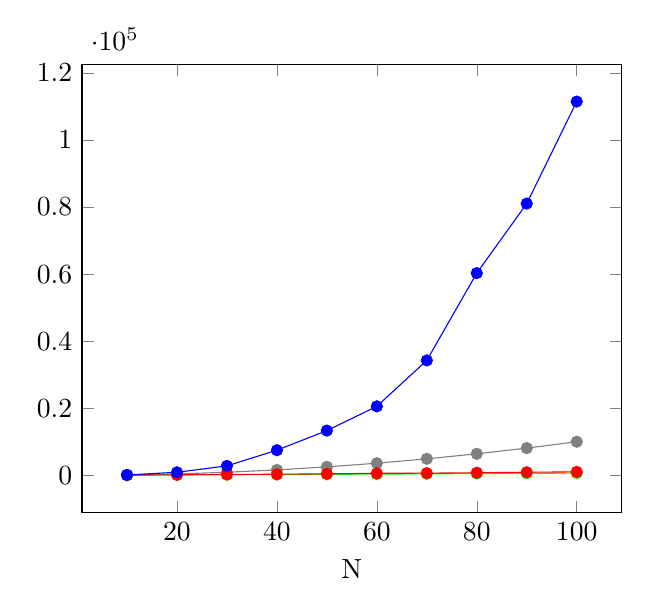
\begin{tikzpicture}
\begin{axis}[xlabel=N]
\addplot [color=gray, mark=*] coordinates{ %squared
  (10,  100)
  (20,  400)
  (30,  900)
  (40,  1600)
  (50,  2500)
  (60,  3600)
  (70,  4900)
  (80,  6400)
  (90,  8100)
  (100, 10000)};
\addplot [color=green, mark=*] coordinates{ %log(n)
  (10,  33.2193)
  (20,  86.4386)
  (30,  147.2067)
  (40,  212.8771)
  (50,  282.1928)
  (60,  354.4134)
  (70,  429.0498)
  (80,  505.7545)
  (90,  584.2668)
  (100, 644.3856)};
\addplot [color=red, mark=*] coordinates{ %quicksort
  (10,  55)
  (20,  134)
  (30,  243)
  (40,  307)
  (50,  436)
  (60,  579)
  (70,  632)
  (80,  750)
  (90,  902)
  (100, 1015)};
\addplot [color=blue, mark=*] coordinates{ %badsort
  (10,  102)
  (20,  890)
  (30,  2799)
  (40,  7480)
  (50,  13321)
  (60,  20557)
  (70,  34266)
  (80,  60294)
  (90,  81034)
  (100, 111456)};
\iffalse
\addplot [color=purple, samples=100, domain=0:10] coordinates{ %cubic
  (10, 1000)
  (20, 8000)
  (30, 27000)
  (40, 64000)
  (50, 125000)
  (60, 216000)
  (70, 343000)
  (80, 512000)
  (90, 729000)
  (100, 1000000)};
\addplot [color=purple, samples=100, domain=0:10] coordinates{ %n^5/2
(10, 316.227766017)
(20, 1788.854382)
(30, 4929.50301755)
(40, 10119.2885125)
(50, 17677.6695297)
(60, 27885.4800927)
(70, 40996.3413002)
(80, 57243.340224)
(90, 76843.3471421)
(100, 100000.0)};
\fi
\end{axis}
\end{tikzpicture}
  \item Draw a conclusion regarding the number of comparisons based on the graph, and draw another conclusion regarding the real execution time from your data collected in part 2b. 
    \begin{itemize}
    \item Looking at the graph of the number of comparisons, I believe badsort to be $\Theta(n^{3})$. If you add in the $n^{3}$ graph (green) and the graph of $n^{5/2}$(red), it closely matches the graph of $n^{5/2}$, but is just a little bit faster growing. From the original graph, it is clear that quicksort is $\Theta(\log{(n)})$ as the lines match fairly perfectly.
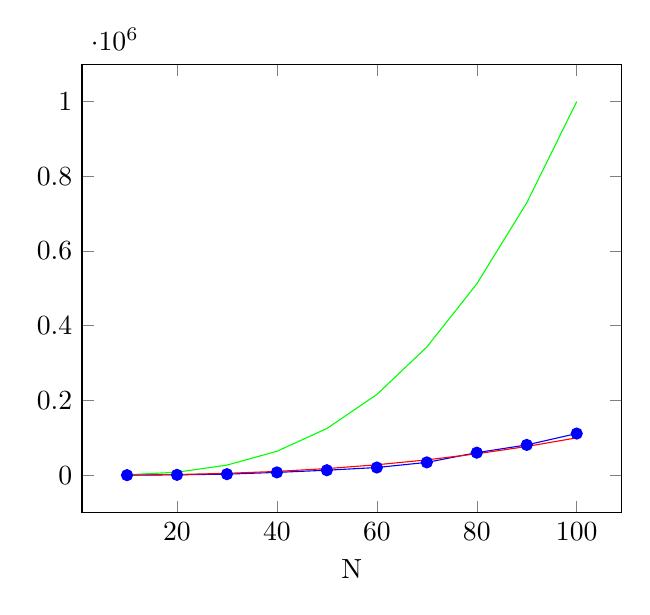
\begin{tikzpicture}
\begin{axis}[xlabel=N]
\addplot [color=blue, mark=*] coordinates{ %badsort
  (10,  102)
  (20,  890)
  (30,  2799)
  (40,  7480)
  (50,  13321)
  (60,  20557)
  (70,  34266)
  (80,  60294)
  (90,  81034)
  (100, 111456)};
\addplot [color=green, samples=100, domain=0:10] coordinates{ %cubic
  (10, 1000)
  (20, 8000)
  (30, 27000)
  (40, 64000)
  (50, 125000)
  (60, 216000)
  (70, 343000)
  (80, 512000)
  (90, 729000)
  (100, 1000000)};
\addplot [color=red, samples=100, domain=0:10] coordinates{ %n^5/2
(10, 316.227766017)
(20, 1788.854382)
(30, 4929.50301755)
(40, 10119.2885125)
(50, 17677.6695297)
(60, 27885.4800927)
(70, 40996.3413002)
(80, 57243.340224)
(90, 76843.3471421)
(100, 100000.0)};
\end{axis}
\end{tikzpicture}
    \item In order to draw a conclusion, we need to look at the economics of the modern computer, the modern supercomputer that is. There exists a single government computer that is powered by two full nuclear power plants, and syphons power from a third coal based power plant. This computer is somewhat open to scientists, and thus this code could possibly be run there if we assume it scales with MPI, which it does if we break our arrays into subsections and then are running bad sort or quicksort on each subarray, which is the normal programming practice. I know that the government computer draws five kilwatts of power while in use and that the wait queue times are directly proportional to the amount of time you want to run. For instance, in order to run for 24 hours on a smaller less used computer, the wait time is about 1 month. So lets assume that running your code uses the full power of the computer, and that each subarray is comparable to what was run, and that performance on each subarray is comparable and requires no extra setup time. In order to run quicksort, you would spend roughly 4 seconds in the queue and your program would run on roughly 0.17651 watts. Badsort on the other hand, would wait in the queue a minimum of 5.67 months in the queue, and use 680.4 kilowatts. We would use all of that, and still not be done sorting our array. I believe from this, its rather obvious to never use the badsort, as most people dont want to spend six months of their lives waiting for something that could take less than five seconds, but if you want to waste 6 months a few thousand watts of electricity, I guess thats up to you.
    \end{itemize}
  \end{enumerate}
\item \textbf{Theoretical Analysis:}
  \begin{enumerate}
  \item Analyze the space complexity for the \textbf{badsort} algorithm.
    \begin{itemize}
    \item The space complexity of the badsort algorithm is $\Theta(1)$. This is due to the algorithm only needing to store the array of n items a constant number of times (zero due to it being passed by reference), and there being nothing else tied to n, such as stack frames if this was a recursive function. You might think that because this function calls swap, and that because swapValues allocates new memory each time it is called, that this should play into the calculations. It does not because although swapValues is in the file, badsort actually calls the standard template library swap function, which does not allocate new memory and operates in constant time.
    \end{itemize}
  \item Analyze the worst-case time complexity for the \textbf{badsort} algorithm. For this part, you will have to \emph{estimate} the total number of object comparisons made by badsort:
    \begin{enumerate}
    \item Try to find a good aymptotic upper bound on the total number of object comparisons made by badsort on an input array of length \emph{n}
      \begin{itemize}
      \item In the worst case, the array is reverse sorted, the outer loop executed n! times.
      \item Using stirlings approximation from earlier in the course, we get $\sqrt{2\pi}n^{n+1/2}e^{-n}$
      \item So the asymtotic upper bound for the worst case is $O=n^{n+1/2}$
      \item In the best case, where the array is sorted, the upper bound is $O(n)$ as it just compares each thing and moves on.
      \item In the average case, we found from our graph that a good upperbound is $O(n^{3})$
      \item As the problem merely asks for an asymptotic upperbound, we must assume the worst case, $O=n^{n+1/2}$
      \end{itemize}
    \item Try to find a good asymptotic lower bound on the total number of object comparisons made by badsort on an input array of length \emph{n} in the \emph{reverse order}.
      \begin{itemize}
      \item Assuming reverse order means sorted from highest to lowest, or reverse sorted, then the asymptotic lower bound is $o=n^{n+1/2}$
      \end{itemize}
    \end{enumerate}
  \end{enumerate}
\end{enumerate}

\subsection{Given C++ code}
\lstinputlisting{Homework/Homework-5/C455-Sp16-Hw5-GivenCode.cpp}
\subsection{My C++ code}
\lstset{language=C++,
	frame=tb,
	showstringspaces=false,
	commentstyle=\color{green},
	keywordstyle=\color{blue},
	stringstyle =\color{red}}
\lstinputlisting{Homework/Homework-5/main.cpp}
\subsection{Makefile}
\lstset{basicstyle=\ttfamily,
        language=bash,
	frame=tb,
	showstringspaces=false,
	commentstyle=\color{green},
	keywordstyle=\color{blue},
	stringstyle =\color{red}}
\lstinputlisting{Homework/Homework-5/Makefile}


% vim: nu expandtab shiftwidth=2 softtabstop=2 foldmethod=marker

\lstset{language=C++,
	frame=tb,
	tabsize=2,
	showstringspaces=false,
	commentstyle=\color{green},
	keywordstyle=\color{blue},
	stringstyle =\color{red}}

\section{Final Exam Guide}

\subsection{Mathematical Tools}
  \begin{itemize}
  \item Definition and properties of floor, ceiling and logarithmic functions
    \begin{enumerate}
    \item floor function
      \begin{itemize}
      \item $\left\lfloor x\right\rfloor$ is an integer
      \item $\left\lfloor x\right\rfloor < x < \left\lfloor x\right\rfloor+1$
      \item $\left\lfloor\sqrt{x}\right\rfloor < \sqrt{x} < \left\lfloor\sqrt{x}\right\rfloor+1$
      \end{itemize}
    \item ceiling function
      \begin{itemize}
      \item $\left\lceil x \right\rceil$ is an integer
      \item $\left\lceil x \right\rceil > x > \left\lceil x \right\rceil-1$
      \item $\left\lceil\sqrt{x}\right\rceil > \sqrt{x} > \left\lceil\sqrt{x}\right\rceil-1$
      \end{itemize}
    \end{enumerate}
  \item Definition and properties of asymptotic notations, focus on: Big-Oh, Big-Omega, and Big-Theta
    \begin{enumerate}
    \item Big-Oh
      \begin{itemize}
      \item $f(n)=O(g(n)) \leftrightarrow$ backwards e constants c, $n_{0}$ $f(n) \leq cg(n)$ for all $n\geq n_{0}$
      \item $\left\lceil\sqrt{n}\right\rceil=O(\sqrt{n})$ because $\left\lceil\sqrt{n}\right\rceil\leq\sqrt{n}+1\leq 2\sqrt{n}$ for all $n\geq 1$
      \end{itemize}
    \item Big-Omega
      \begin{itemize}
      \item $f(n)=Ohmega(g(n)) \leftrightarrow$ backwards e constants c, $n_{0}$ $f(n) \leq cg(n)$ for all $n\geq n_{0}$
      \item $\left\lceil\sqrt{n}\right\rceil=Ohmega(\sqrt{n})$ because $\left\lceil\sqrt{n}\right\rceil\leq\sqrt{n}+1$ for all $n\geq 1$
      \item Then $\left\lceil\sqrt{n}\right\rceil=\Theta(\sqrt{n})$
      \end{itemize}
    \item Big-Theta
    \end{enumerate}
  \item Recognize linear recurrence relations and its components (coefficients, nonhomogeneous terms)
  \item Methods to solve recurrence relations (characteristic equation, backward substitution). How and when to use those methods?
  \item Definition and properties of binary trees.
    \begin{itemize}
    \item Height of a tree with n nodes
      \begin{itemize}
      \item minimum $\left\lfloor\log{(n)}\right\rfloor$ (when the tree is balanced)
      \item maximum $n-1$ (when it is in a straight line
      \end{itemize}
    \item Number of empty subtrees in a tree with n nodes is n+1
    \item Number of leaves in a tree with n nodes is
      \begin{itemize}
      \item minimum 1 leaf
      \item maximum $\left\lfloor\frac{n}{2}\right\rfloor$
      \end{itemize}
    \end{itemize}
  \end{itemize}
\subsection{Algorithm Analysis}
  \begin{itemize}
  \item How to count the number of iterations of a single loop, and  nested loops? (See sample questions in page 2 below)
  \item How to analyze worst case space complexity of a function call
    \begin{itemize}
    \item To analyze space complexity, Two things you need to mention are
      \begin{enumerate}
      \item [1] The size of each stack frame.
      \item [2] The maximum number of stack frames on the runtime stack
      \end{enumerate}
    \end{itemize}
  \item How to analyze the best case \& worst case time complexities of an algorithm
    \begin{itemize}
    \item [***Note***] this is a focus of the exam, use the below as an example
    \item Best Case time complexity $T(n)$ of an algorithm is the minimum running of that algorithm on any input of size n
    \item Worst Case time complexity $T(n)$ of an algorithm is the maximum running of that algorithm on any input of size n
    \end{itemize}
  \item Understand the deterministic analysis of the following algorithms:
    \begin{itemize}
    \item Euclid's GCD
    \item linear search
    \item binary search
    \item merge--sort
    \item quicksort
    \item binary tree traversal (print in order)
    \item searching a binary search tree
    \item insert a new node into a binary search tree
    \end{itemize}
  \item Understand the theorem for the lower bound of comparison-based sorting algorithms (Theorem 5.9.1 in the textbook)
    \begin{itemize}
    \item [***Note***] not a focus of the exam
    \item Need to understand what it implies in the slides
    \item Exercise $5.9.5$ in the textbook pages $278-279$ the answer is no for a because they use the word always.
    \item The theory is only for the lower bound on the worst case time complexity of any comparison based sorting algorithm
    \end{itemize}
  \item Understand the probabilistic analysis of the following algorithms:
    \begin{itemize}
    \item [***NOTE***] only one big thing you need to remember is that in order to perform average case analysis for any algorithm.
    \item I was correct that you use induction for this if you want.
      \begin{itemize}
      \item Assume the input is random
      \item Estimate the expected running time of the algorithm
      \end{itemize}
    \item linear search
    \item quicksort
    \end{itemize}
  \end{itemize}
\subsection{sample questions}
\begin{enumerate}
\item How many times does the word ``Hi'' is printed out by the following loop, assuming variable n has been declared and given an arbitrary positive integer?
  \begin{lstlisting}
for (i=1; i*i<=n; i++)
  cout << "Hi";
  \end{lstlisting}
  \begin{enumerate}
  \item n
  \item $\left\lfloor\sqrt{n}\right\rfloor$
  \item $n\left\lfloor\sqrt{n}\right\rfloor$
  \item $n^{2}$
  \end{enumerate}
\item How many times does the word ``Hi'' is printed out by the following loop, assuming variable n has been declared and given an arbitrary positive integer?
  \begin{lstlisting}
for (i=1, k=n; i<n; i++, k=k/2)
  for (j=0; j<k; j++)
    cout << "Hi";
  \end{lstlisting}
  \begin{enumerate}
  \item $\sum\limits_{i=0}^{n-1}\left\lfloor\frac{n}{2^{i}}\right\rfloor$
  \item n
  \item $\frac{n}{2}$
  \item $n^{2}$
  \end{enumerate}
\end{enumerate}

\end{document}
